\section{Heat-Exchangers}
\quad\ One of the last component that had to be modeled was the heat-exchanger. The purpose of an heat-exchanger is to exchange energy from one flow to the other using heat transfer. 

To model the heat-exchanger, the relations characterizing the heat transfer from a hot flow (H) to a cold flow (C) needs to be implemented. To recall those relations described in the chapter \ref{C4}, the relations (\ref{eq:C7_Qdot}), (\ref{eq:C7_Qmax}),  (\ref{eq:C7_QdotQmax}) respectively describes the actual heat transfer rate from the hot flow to the cold flow, the theoretical maximal heat transfer rate, and the relation between these two quantities.   

\begin{subequations}
\setstretch{1}
\begin{align}
    \dot{Q} &= \dot{C}_C\cdot (T_{C,out} - T_{C,in}) = \dot{C}_H\cdot(T_{H,in} - T_{H,out})\label{eq:C7_Qdot}\\
    \dot{Q}_{max} &= \dot{C}_{min}\cdot (T_{H,in} - T_{C,in})\label{eq:C7_Qmax}\\
    \dot{Q} &= \varepsilon\cdot\dot{Q}_{max}\label{eq:C7_QdotQmax}
\end{align}
\end{subequations}
Where $\dot{C} = \dot{m}\cdot c_p$ is thermal heat capacity, and the index "in" and "out" specifies if the temperature is taken at the entrance or the outlet of the heat-exchanger. 

Based on how the heat-exchanger to be modeled is defined, the usage of these relations will vary. For instance, for a water heat-exchanger the inlet and outlet temperature of the water to be heat-up are usually known before the computation. Indeed, for this application it is important to maintain at least the outlet temperature constant to provide a reliable heating system. 

These variations are going to be described in the following parts of this section.

\subsection{Regenerator}
\quad\ First are considered the regenerator. The purpose of this category of heat-exchanger is to preheat a cold flow of a cycle using the hot flow coming from a different stage of the same cycle. This usually increases the thermal efficiency $\eta$ of the system\footnote{see the chapter \ref{C5} for more information}. The thermal efficiency $\eta$ is defined as being the ratio between the net work output of the system and the amount of energy transfer to the fluid in the combustion chamber. 

For the modeling of this first category of heat-exchanger, the inlet temperature and the mass flow rate of both flows are known. Therefore, the maximal heat transfer rate  $\dot{Q}_{max}$ can be easily computed by applying the equation \ref{eq:C7_Qmax}. By calculating the minimal thermal heat capacity $\dot{C}_{min}$ defines as being the minimum between $\dot{C}_H$ and $\dot{C}_C$, $\dot{Q}_{max}$ can be obtained.

From there, the actual heat transfer rate $\dot{Q}$ can be computing using the relation (\ref{eq:C7_QdotQmax}). $\varepsilon$ is the thermal efficiency of the heat-exchanger. In the event where the efficiency is assumed to be independent of the operating condition of the heat-exchanger, a constant value is used. In reality the thermal efficiency of the heat-exchanger depends on the temperature and the mass flow rate of the flows. The method to take into account this dependency will be described later in this section.

Then, once the heat transfer rate $\dot{Q}$ is computed, the temperatures $T_{H,out}$ and $T_{C,out}$ at the outlet of the heat-exchanger is computed using the formulas in (\ref{eq:C7_Qdot}).

\subsection{Water heat-exchanger and inter-cooler}
\quad\ Now are considered the water heat-exchanger (WHX). As it has been mentioned previously, the purpose is to use the energy within the gas to heat-up water. This water is used for sanitary purposes or to feed an heating system (like in a house). 

It is often required for this type of application that the outlet temperature of the water remains constant. Indeed, this outlet temperature corresponds to the starting temperature of the water into the auxiliary loop. Thus, it is preferable to have steady condition in times for the outlet state of the water.

In this model of the Brayton cycle, the inlet temperature of the water is fixed as well. This implies that the only degree of freedom is on the mass flow rate of the water within the water heat-exchanger. The Figure \ref{fig:C7_WHX} depicts a schematic of a water heat-exchanger.

\begin{figure}[h]
    \centering
    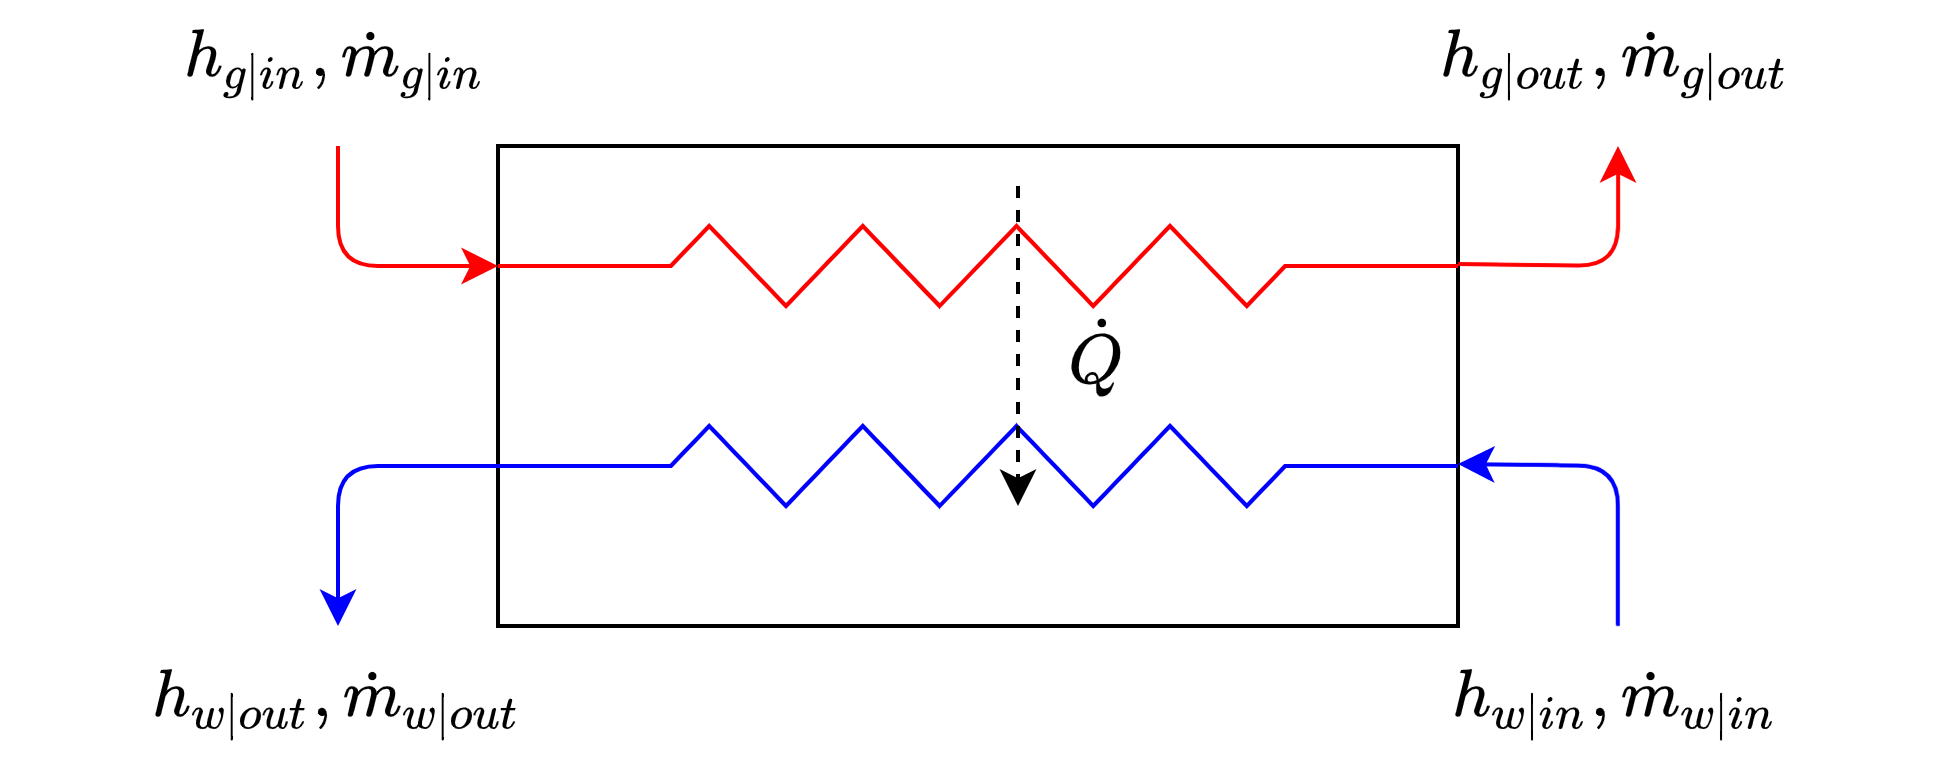
\includegraphics[width=0.6\textwidth]{Chapitre_7/Images/WHX.png}
    \caption{Schematic of a water heat-exchanger}
    \label{fig:C7_WHX}
\end{figure}

Therefore, the known variables are the inlet temperature $T_{g,in}$ and the mass flow rate $\dot{m}_g$ for the gas of the cycle, and the inlet and outlet temperature for the water. Since the mass flow rate of the water is a unknown, an iterative process need to be made. 

Starting from the second relation (\ref{eq:C7_Qmax}), the theoretical heat transfer rate $\dot{Q}_{max}$ can be estimated based on the initial guess for the mass flow rate of water $\dot{m}_w$. Then, the heat transfer rate $\dot{Q}$ is obtained using the third relation (\ref{eq:C7_QdotQmax}). 

Once $\dot{Q}$ is computed, the guess on the mass flow rate $\dot{m}_w$ can be updated considering the first relation (\ref{eq:C7_Qdot}). Indeed, the term of the relation can be reorganized to obtain the relation (\ref{eq:C7_mupd}) that will update the value of the mass flow rate of water.

\begin{equation}
    \setstretch{1}
    \dot{m}_w = \frac{\dot{Q}}{c_{p,w}\cdot \left(T_{w,out} - T_{w,in}\right)} \label{eq:C7_mupd}
\end{equation}

In addition to the water heat-exchangers that use the heat from the hot exhaust gas, water heat-exchangers are also used when the the compression is split into several stages. Between each of these stage, the air is watercooled in order to reduce its temperature before the next stage of compression. For this specific application, the heat-exchangers is called intercooler.

\subsection{Variable efficiency}
\quad\ It has been mentioned before that the thermal efficiency of the heat-exchanger varies with the operating conditions. In chapter \ref{C4}, some mathematical derivations have been to obtain the formulation (\ref{eq:C7_hconv}) for the convective heat transfer coefficient $h_{conv}$ of the flow. 

\begin{equation}
    \setstretch{1}
    h_{conv} = 0.0697\cdot \frac{\dot{m}^{4/5}\cdot c_p^{1/3}}{\pi^{4/5}\cdot D^{9/5}}\cdot \frac{\lambda_c^{2/3}}{\mu^{7/15}}\label{eq:C7_hconv}
\end{equation}

This relation involved the calculation of the heat conductivity $\lambda_c$ and the dynamic viscosity $\mu$. The method to compute these state variables has been presented in the first section of the chapter \ref{C7}.

Also, the diameter of the duct is involved in the relation. However, by making the assumption that the geometry of the cold and hot side of the heat-exchanger are really closed from one to the other, the knowledge of the diameter $D$ is not required anymore. Similarly, the constant 0.0697 and $\pi^{4/5}$ are not required for the following derivation. Therefore, the reduced relation (\ref{eq:C7_hconvred}) is used instead.

\begin{equation}
    \setstretch{1}
    h_{conv} = \dot{m}^{4/5}\cdot c_p^{1/3}\cdot \frac{\lambda_c^{2/3}}{\mu^{7/15}}\label{eq:C7_hconvred}
\end{equation}

Considering first the nominal condition specified in the data, the nominal convective heat transfer coefficients $h_{conv,H}$ nad $h_{conv,C}$ can be obtained using the relation (\ref{eq:C7_hconvred}). From this, the nominal heat transfer coefficient $U_{nom}$ is computed based on the definition (\ref{eq:C7_U}).

\begin{equation}
    \setstretch{1}
    U = \frac{h_{conv,H}\cdot h_{conv,C}}{h_{conv,H} + h_{conv,C}}\label{eq:C7_U}
\end{equation}

From the nominal conditions, it is also know the nominal efficiency $\varepsilon_{nom}$ of the heat-exchanger. With the ratio $C_{r,nom}$ of the nominal heat transfer capacity $\dot{C}_{min,nom}$ and $\dot{C}_{min,nom}$, the nominal number of transfer unit NTU$_{nom}$ can be computed by applying the formula (\ref{eq:C7_eps}).

\begin{align}
    \setstretch{1}
    \varepsilon = \frac{1 - e^{-\text{NTU}\cdot (1 - C_r)}}{1 - C_r\cdot e^{-\text{NTU}\cdot (1 - C_r)}}\label{eq:C7_eps}
\end{align}

Once the nominal number of transfer unit NTU$_{nom}$ obtained, the global area $A$ of the heat-exchanger is obtained based on the definition (\ref{eq:C7_NTU}) of the number of transfer unit.

\begin{equation}
    \setstretch{1}
    \text{NTU} = \frac{A\cdot U}{\dot{C}_{min}} \label{eq:C7_NTU}
\end{equation}

The efficiency $\varepsilon$ of the heat-exchanger can now be obtained for the non nominal operating conditions. By computing the heat transfer coefficient $U$, the number of transfer unit NTU is easily obtained. Then, the relation \ref{eq:C7_eps} will provide the efficiency of the heat-exchanger when the operating conditions are not the nominal ones.